\fancychapter{EMYS: the \emph{Sueca} player}
\label{chapter:approach}

Revising the purposes of this work, presented in Section~\ref{sec:goals}, the robotic agent that plays \emph{Sueca} has two main tasks: to choose an adequate card to play and to interact socially according to the game state.
In order to achieve these goals, some state-of-the-art approaches have been reviewed and considered for the implementation in our domain.
Thus the current chapter aims to carefully describe the decisions that were taken, some limitations imposed by the domain, as well as enhancements that have been made.
It starts with an overview of the whole system, proceeds with the implementation of the artificial player and last of all, details the development of the social agent.

\section{Architecture Overview}
\label{section:architecture_overview}

The model presented in Figure~\ref{fig:model} organises all the components involved in this system and their communications.
It considers a scenario where an embodied agent plays a physical card game against human players over a touch table.

\begin{figure}[ht]
  \centering
    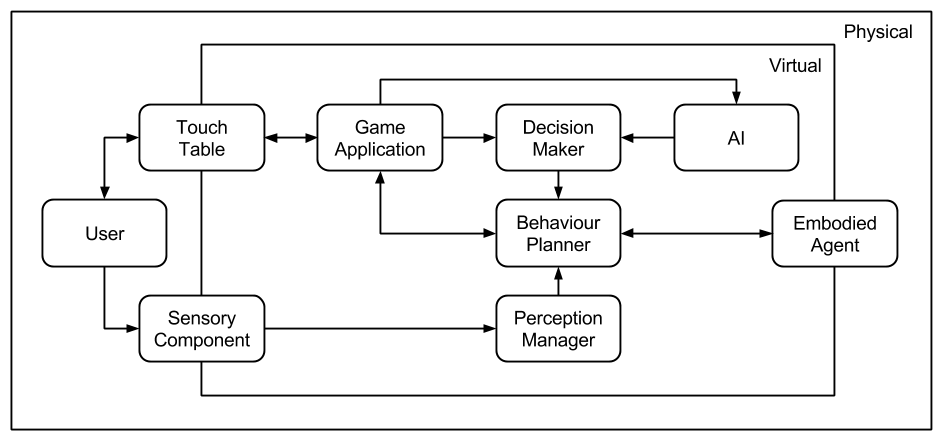
\includegraphics[width=1\textwidth]{./img/architecture}
  \caption{System architecture using components}
\label{fig:architecture}
\end{figure}

First of all, this model distinguishes physical components from virtual ones.
However, some entities are presented as both physical and virtual components and will not be detailed since their usage in this system did not demand any extensions for the scope of our domain (\emph{Touch Table}, \emph{Sensory Component} and \emph{Embodied Agent}).

The basic work-flow that illustrates the main functionalities of each component is as follows.
The human players, \emph{Users}, play with physical cards on top of a \emph{Touch Table}, and their game actions are managed by the \emph{Game Application} and communicated to both the \emph{\ac{ai}} and the \emph{Decision Maker}.
\todo[inline]{check the sensory components!}
Besides their game actions, \emph{Users} also produce another sort of events that are captured by the \emph{Sensory Component} and handled by the \emph{Perception Manager}, for instance, face movements or the source direction of spoken interactions.
The \emph{\ac{ai}} includes all the reasoning about the game and decides the next move of the artificial player.
However, the \emph{Embodied Agent} will not only play a certain card, but will also include social behaviours.
As a result, the \emph{Decision Maker} balances the \emph{\ac{ai}} decisions and game information to produce an appropriate sequence of behaviours and inform them to \emph{Behaviour Planner}.
Lastly, the \emph{Behaviour Planner}, after receiving high-level intention-directed instructions, builds a suitable plan to execute the chosen instructions, considering the state of the \emph{Embodied Agent}, information from \emph{Perception Manager}, and additional game information from the \emph{Game Application}.

\begin{figure}[ht]
  \centering
    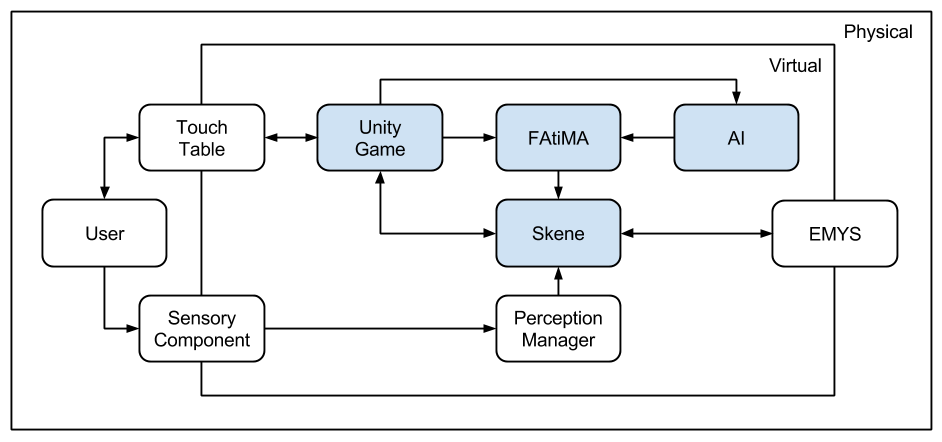
\includegraphics[width=1\textwidth]{./img/model}
  \caption{System architecture using modules}
\label{fig:model}
\end{figure}

\todo[inline]{confirmar com o Tiago se sai uma seta do skene para o unity!!!}
The previously described architecture is instantiated as shown in Figure~\ref{fig:model} and the blue modules are thalamus communicating entities.
This concept arises from the Thalamus Framework \cite{Ribeiro}, which enables the usage of entities that can be registered at runtime in a server in order to send and receive specific messages.
These entities are publishers and subscribers of the channels they want to write on and listen to, respectively.
The implementation provided by this framework works by simply inherit from the \emph{ThalamusClient} class and implement the interfaces of the messages that the entity wants to exchange.

The \emph{Unity Game} module is responsible for displaying the interface of the game, reading the physical cards, publishing all the relevant game events and subscribing to the plays of artificial players.

The chosen \emph{Behaviour Planner} is \emph{Skene} \cite{Ribeiroa}, which tightens the communication between the world and an embodied agent with a high-level behaviour description language, also known as utterances.
These utterances might include instructions for gazing, pointing, animating or sound, among other things.
Additionally, considering some instructions require target positions or other game information, Skene subscribes to \emph{Unity game} messages to keep that information updated.

The \emph{\ac{ai}} and \emph{FAtiMA} modules answer to our primary goals, for that reason, their implementations are carefully detailed in Section~\ref{sec:artificial_player} and Section~\ref{sec:social_player}, respectively.

\section{An intelligent player}%The artificial player}
\label{sec:artificial_player}

This section will describe the most relevant implementation details of the artificial player.
After thoroughly analysing state-of-the-art techniques to solve imperfect information games, and considering \emph{Sueca} is, at this moment, computationally unsolved, the chosen approach was \ac{pimc}.
To implement this search technique, there are three key concepts or algorithms that require a full understanding: the Information Set, the PICM Search and the MinMax Algorithm.
Moreover, the encountered drawbacks are also further described, as well as the enhancements implemented to overcome those limitations.

\subsection*{Information Set}

An information set represents all the visible information during a game, and also inferred information based on certain events.
The player must keep an instance of the information set per game and update it when necessary.
It stores the known hand of the player and a deck with all the cards whose owner is unknown.
As a result, each time another player plays a card, it should be removed from that deck.

The purpose of managing unplayed cards is to sample possible card distributions for the other three players with their real conditions.
These sampled distributions will be used during the \ac{pimc} search and the closer they are to the real world, the better the search returning value will be.
Additionally, the information set keeps track of suits per player and, when a player does not follow the leadsuit of a trick, it removes that suit from the player possible suits.
By possessing this information, sampling possible distributions gets closer to the real world, however it increases the complexity of the sampling process.
The sampling method builds a \ac{csp} where:
\begin{itemize}
\item variables are the unplayed cards;
\item each domain is the set of players that still have that suit;
\item and the constraints are the number of times a player can be assigned to a card.
\end{itemize}


\subsection*{\ac{pimc} Search}

The following pseudo-code of the \ac{pimc} search algorithm guided the implementation.

\begin{algorithm}
	\caption{PIMC search algorithm}
	\begin{algorithmic}[1]
		\Procedure{PIMC}{InfoSet $I$, int $N$}
			\ForAll {$m \in$ Moves($I$)}
				\State $val[m]$ = 0
			\EndFor
			\ForAll {$i \in \{ 1..N\}$}
				\State $x$ = Sample($I$)
				\ForAll {$m \in$ Moves($I$)}
					\State $val[m]$ += PerfInfoValue($x$, $m$)
				\EndFor
			\EndFor
			\State \textbf{return} $\underset{m}{argmax}\{ val[m] \}$
		\EndProcedure
	\end{algorithmic}
\end{algorithm}

To recapitulate the main points of this algorithm, considering it can choose up to \#Moves($I$), it samples $N$ possible card distributions for the other three players and calculates the reward of playing each possible move for the $N$ sampled worlds.
The returned move is the one that gave more accumulated reward.

The number of iterations this algorithm perform is imposed by the $N$ parameter.
Another version of the algorithm, instead of limiting the number of iterations, specifies the execution time of the main loop.

\subsection*{MinMax Algorithm}

As mentioned above, \ac{pimc} has to calculate the reward of playing a card, for each sampled world.
Since a sampled distribution assigns the remaining cards to the players, every game can be handled as a perfect information game.
Therefore, to compute a perfect information game, considering each player or team intends to win, the MinMax algorithm was used.

MinMax is a popular algorithm for calculating optimal decisions in multiplayer games.
Each node corresponds to a possible move by a player and their successors correspond to the possible moves of the next player.
The player representing \ac{emys} and his team mate are both max players, likewise, the other two opponents are min players.

The complete game tree has 40 levels, from $l_{0}$ to $l_{39}$, and each group of $l_{4n}$ to $l_{4n+3}$ represents a trick.
Additionally, since the utility value can only be determined in terminal nodes, these back-propagate their best or worst child utilities, if they are max or min nodes, respectively.
The chosen utility function to evaluate a game is the winning team score, a positive value when the agent team wins and a negative value otherwise.
\todo[inline]{rever a utility function de acordo com a avaliacao}



\subsection{Drawbacks and enhancements}

When applying \ac{pimc} to decide which move to make, the number of computed game trees is \#Moves($I$) times $N$ (the number of different distributions), and the size of a game tree depends on the moves that are left to finish the game.
Additionally, the algorithm tends to choose a near optimal decision as long as the $N$ is reasonably large.
As a result, this algorithm has to process a large number of nodes to make a proper decision, specially in the beginning of the game, and, without the enhancements further described, this task was impractical.

\citet*{Russell2009} suggested that MinMax performance can be improved using the alpha-beta prunning, a move ordering heuristic, and a transposition table.
The alpha-beta prunning, by simply storing the best choices so far for the max and min nodes, does not explore nodes that will not influence the final decision.

This technique can also be improved with a favourable ordering heuristic that produces earlier alpha-beta cuts.
Therefore, the implemented ordering heuristic is dynamic and uses an auxiliary computation to decide how to order moves.
Similarly to a human player reasoning, it analyses the current trick and tries to anticipate its winner.
If this auxiliary procedure expects the winner to be one of its opponents, it orders the cards from the less valuable to the most valuable, otherwise, it does the opposite.
This concept might appear as a hard trade-off between the produced speed and the time spent on this extra computation plus the sort.
However, alpha-beta cuts have reasonably increased and reduced significantly the exploration time of the whole tree.

Another improvement with remarkable results on the MinMax performance was a transposition table.
Considering each card configuration or distribution will produce \#Moves($I$) game trees, they will contain sufficient similar subtrees to store their first computed values.
Therefore, instead of recomputing them, they can be reused.

Furthermore, another heuristic was used, aiming to reduce redundancy in the state generation, suggested by \citet{Buro}.
When computing Moves($I$), two or more cards of the same suit, with consecutive ranks and with the same value can be considered as the same move, since they produces the same value.
For instance, holding 3$\clubsuit$, 4$\clubsuit$ and 5$\clubsuit$ on the same hand will produce three equivalent states and therefore, this heuristic produce only one.

Limiting the maximum depth achieved by the MinMax algorithm was another available option, specially for earlier decisions that produce larger trees.
However, considering a non-terminal node as terminal implies the utility function must be revised or predicted.
For that reason, when limiting the search depth, the following utility function was used:
\todo[inline]{Utility function for depth limit MinMax and based on analysed games!}

Lastly, to exploit the computational resources and considering the fact that \ac{pimc} can be easily paralleled, the outer loop was divided into the number of \acp{cpu} the machine has.
Using a machine with 4 \acp{cpu}, the speed-up is nearly 4.
The only concern while paralleling this algorithm is to carefully manage the scope of shared and private variables among the threads.
















\section{A social player}
\label{sec:social_player}

First of all, a social player in a card game scenario is basically a player that can interact with other human players in a proper way according to the game situation.
Since its behaviours must be as similar as possible to the interactions of human players, the most expressive robot was chosen to embody this player, \ac{emys}.
Nevertheless, when creating behaviours for an embodied agent, it is important to consider that our perception of a social robot, as a unique entity that interact, is indeed composed of distinct modules that make the robot talk, move, animate, gaze at some point or glance at another.
For this reason, the architecture, presented in Figure\ref{fig:model}, uses \emph{Skene} as its \emph{Behaviour Planner}.
\emph{Skene} has its own language, called utterances, that allow the communication with the robot as a single entity.
These utterances are classified with a category and subcategory and may specify verbal or non-verbal behaviours, as well as both interleaved.
Most of \ac{emys} behaviours in this scenario were conducted by \emph{Skene} due to the provided abstraction while producing complete behaviours (verbal and non-verbal), and also due to the utterances classification that can associate behaviours to game states.
The current section will present the main aspects of the utterances list that characterizes \ac{emys} behaviours and the way it will be perceived.
%However, invoking specific instructions without \emph{Skene} can also be directly done

%Additionally, a \emph{Sueca} player has two distinct roles during a game: being partner of his team player and opponent of the other two players.
%With these main concepts in mind, a character of this nature can be developed by specifying its behaviours.
%In other words, considering the connection between the world and the robot is established by \emph{Skene}, this means creating a list of utterances that might contain text to speak, animations, gaze and glance instructions.
%The current section describes the structure of behaviours included in the developed \emph{Sueca} player.


\subsection{\emph{Sueca} behaviours}
The analysis of the card game players on user centred studies revealed key aspects of the interaction during a \emph{Sueca} game.
First of all, there are specific game situations that may cause verbal or non-verbal behaviours.
As a result, these game situations guided the categories and subcategories of the utterances list, presented on the following figure.

\begin{figure}[ht]
	\centering
    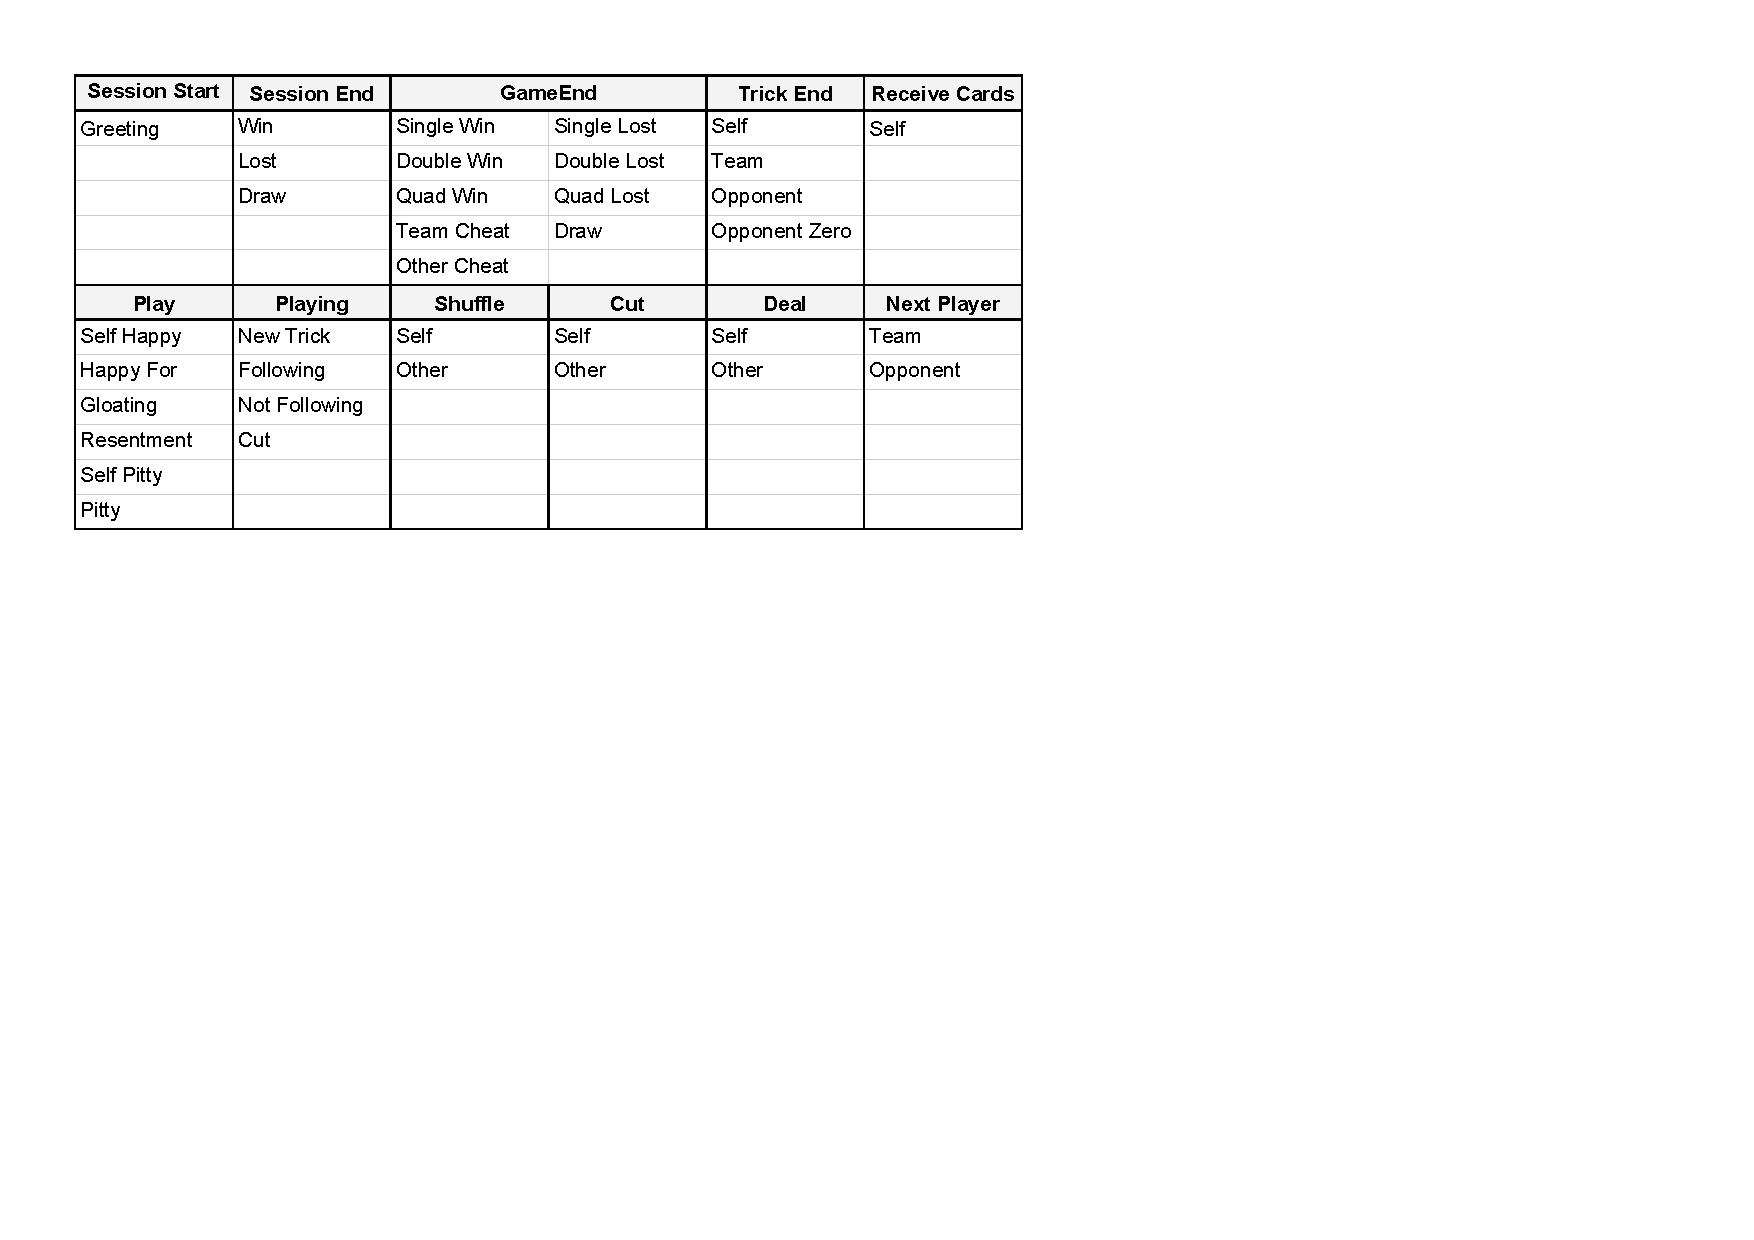
\includegraphics[width=1\textwidth]{./img/utterances}
	\caption{Categories and subtegories of the utterances list}
\label{fig:utterances}
\end{figure}

The final list of 205 distinct utterances was inspired by the collected behaviours and replicated to similar ones in order to enrich interactions and to avoid speech redundancies.
The annotated non-verbal behaviours were also applied on \emph{emys} during the same game situations, for instance, looking at a played card and analysing its own hand after that, simulating a re-evaluation of the game.

\subsection{Human-like behaviours}

Besides simply replicating behaviours from human players, there are other things to consider in order to make the robot act as a human, for instance, its speech frequency or its emotional state.
Consequently, this social player applies a probability to decide whether or not to perform an utterance for each game situation.
Additionally, a \emph{FAtiMA} module was used, as shown in Figure~\ref{fig:model}, to enrich \ac{emys} presence and allow it to share its emotional state.

\emph{FAtiMA} is a modular architecture for an emotional agent capable of producing 22 different emotions based on its goals and its perceptions of new events for a determined scenario.
Perceptions can be updated by changing the values of 6 appraisal variables (desirability, desirability for other, success probability, failure probability, praiseworthiness and like) and their combination can generate one or more emotions.
However, the current emotional agent of this \emph{Sueca} player is only using 4 appraisal variables, which means it only produces 12 emotions, as presented in Figure~\ref{fig:emotions}

\begin{figure}[ht]
	\centering
    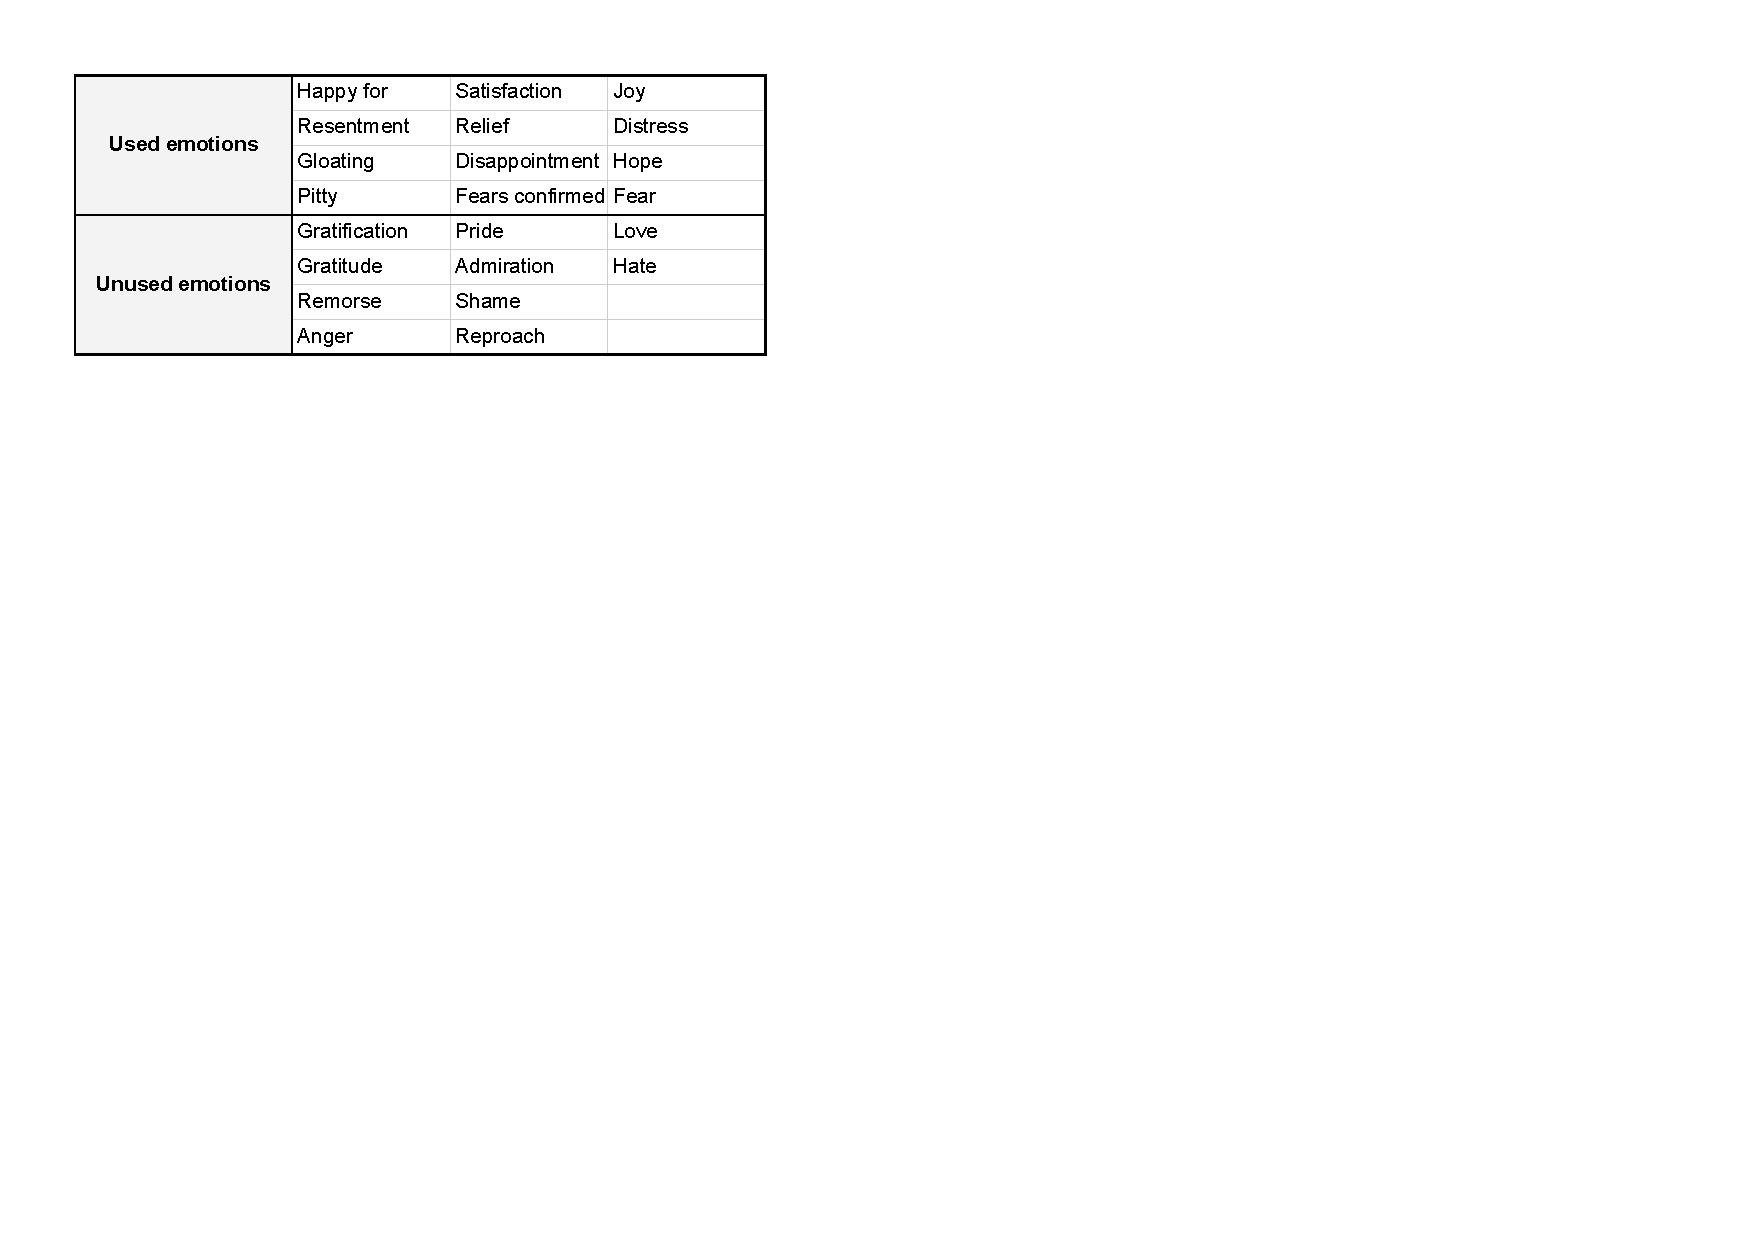
\includegraphics[width=1\textwidth]{./img/emotions}
	\caption{FAtiMA emotions divided}
\label{fig:emotions}
\end{figure}

These emotional states could have been used to subcategorize utterances, however, the analysis of humans playing \emph{Sueca} evidenced their behaviours mostly depend on the specifications of a certain move or simply sign 

frequency
emotions

\subsection{Enhancing the game interface with behaviours}
nextplayer
receiving cards
trick end

\clearpage

